%!TEX root=main.tex
\section{引言}

本章的主题是网络虚拟化和网络功能加速,在本文中的位置如图 \ref{clicknp:fig:sys-arch} 所示。

\begin{figure}[htbp]
	\centering
	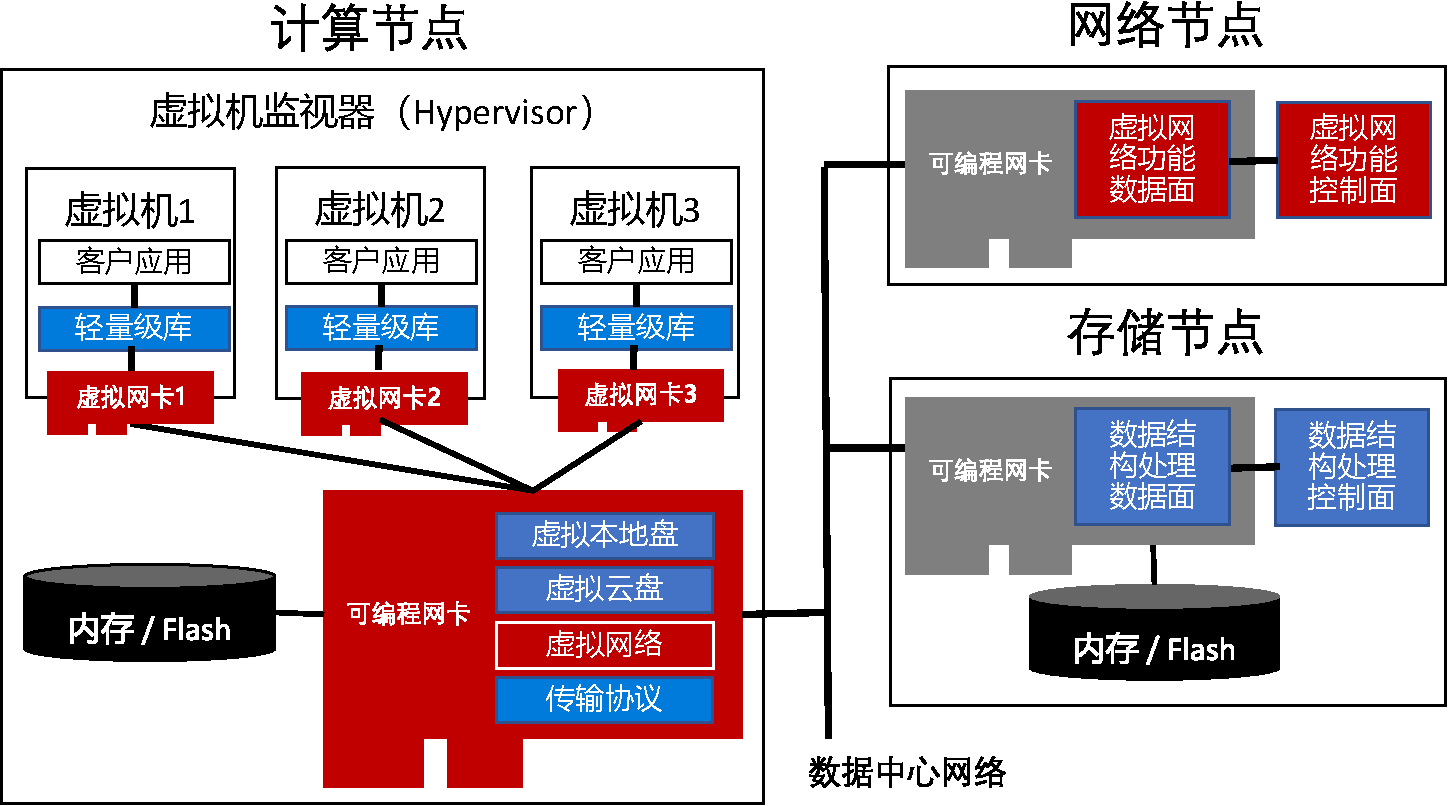
\includegraphics[width=0.8\textwidth]{image/sys_arch.pdf}
	\caption{本章主题:网络虚拟化和网络功能加速,用红色标出。}
	\label{clicknp:fig:sys-arch}
\end{figure}

本章作为全文的基础,将提出一个 FPGA 高级语言编程框架,以及主机 CPU 上相应的运行时,并在此基础上实现硬件加速的网络功能,如图 \ref{clicknp:fig:sw-hw-codesign} 所示。

\begin{figure}[htbp]
	\centering
	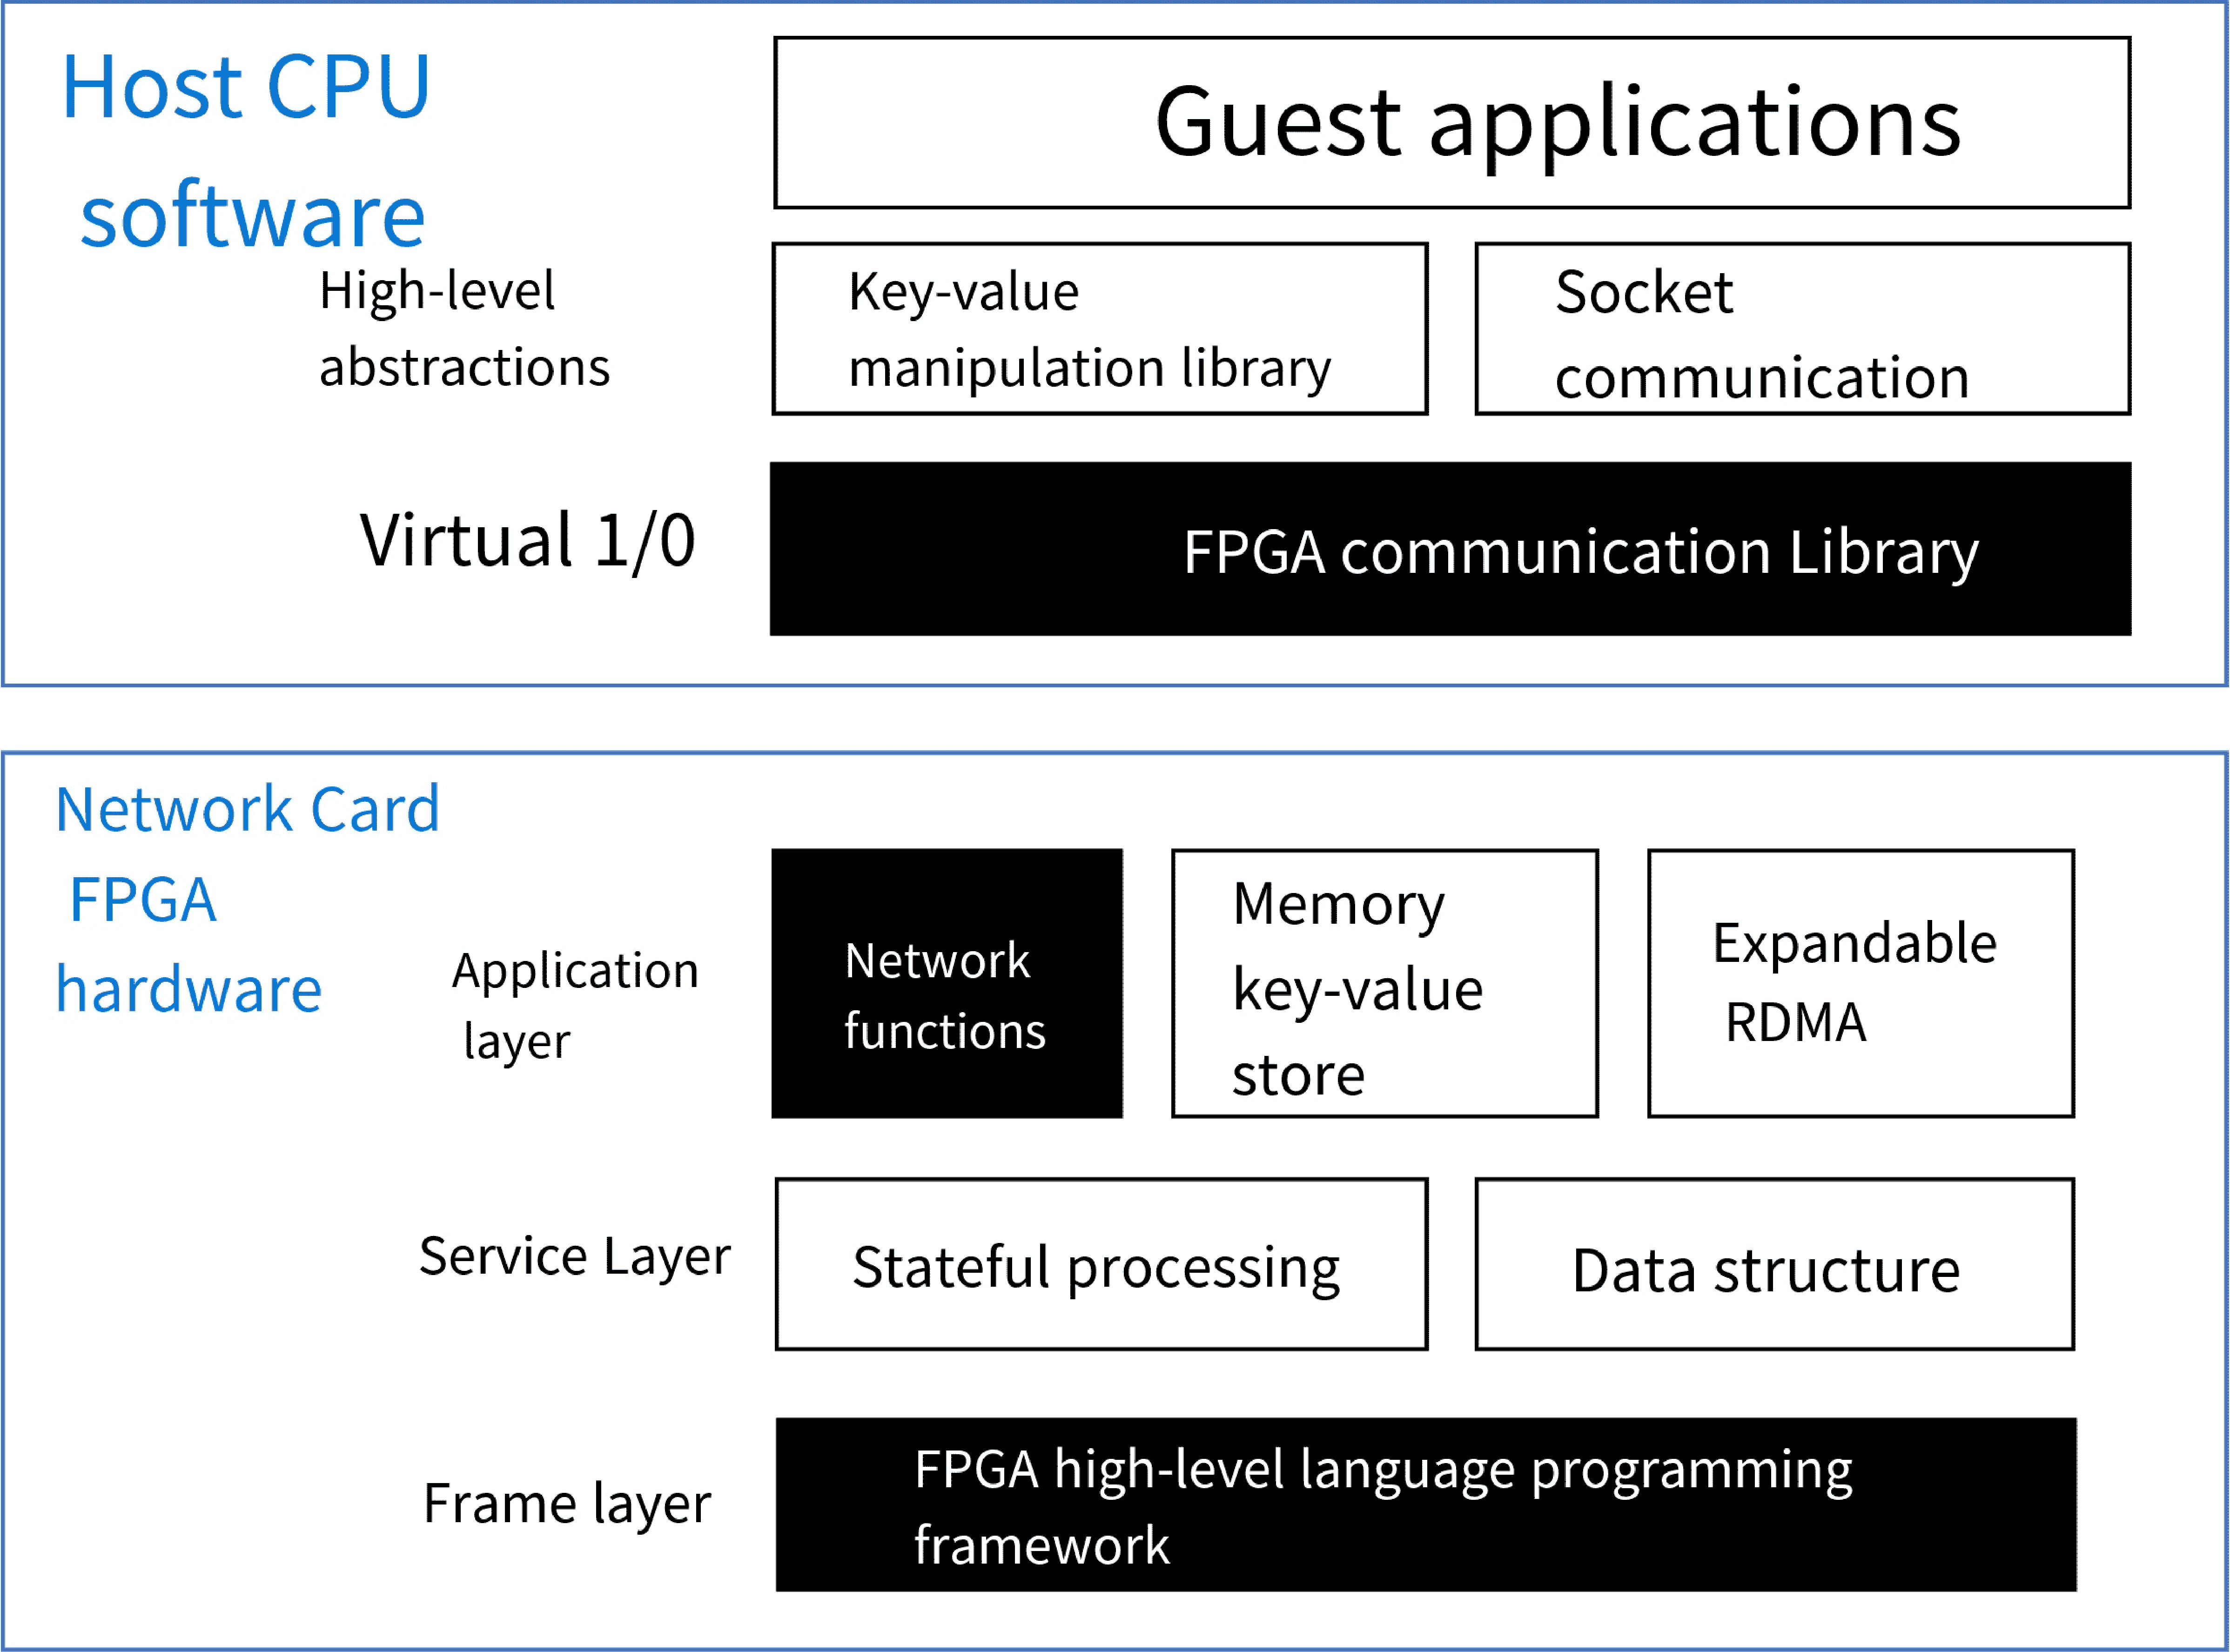
\includegraphics[width=0.5\textwidth]{image/sw_hw_codesign.pdf}
	\caption{本章在可编程网卡软硬件架构中的位置。}
	\label{clicknp:fig:sw-hw-codesign}
\end{figure}

现代多租户数据中心提供共享基础设施,以低成本托管来自不同客户(即租户)的许多不同类型的服务。
为确保安全性和性能隔离,每个租户都部署在\textit{虚拟化网络}环境中。
数据中心运营商需要灵活的网络功能(Network Function,网络功能)来实施隔离
同时保证服务水平协议(Service Level Aggrement,SLA)。

传统的基于硬件的网络设备不灵活,因此几乎所有现有的云提供商,例如Microsoft,Amazon和VMWare,已经在服务器上的管理程序软件中实现了\textit{虚拟化}网络功能,以最大限度地提高灵活性,包括负载均衡、流量整形和防火墙等。

但是,软件网络功能有两个基本限制 - 都源于软件包处理的性质。
首先,用软件处理数据包的容量有限。
现有的软件网络功能通常需要多个内核来实现10~Gbps的速率~\cite{comb,martins2014clickos}。
但最新的网络链接已经扩大到40至100~Gbps~\cite{mellanox-100g}。
虽然可以在服务器中添加更多内核,但这样做会增加成本,不仅在资本支出方面,而且在运营费用增加时会产生更多的能源。
%
其次,在软件中处理数据包会产生大量且高度可变的延迟。 这种延迟的范围可能
从几十微秒到几毫秒~\cite{martins2014clickos,ananta,duet}。
对于许多低延迟应用(例如,股票交易),这种增加的延迟是不可接受的。

% hardware accelerating
为了克服软件包处理的局限性同时保持灵活性,最近的工作已经提出使用图形处理单元(GPU)~\cite{packetshader},网络处理器(NP)~\cite {cavium,netronome}或可重新配置的硬件(现场可编程门阵列,即FPGA)来加速网络功能~\cite{netfpga,smartnic,rubow2010chimpp}。
与GPU相比,FPGA更节能~\cite {fpga-vs-gpu,fpga-vs-gpu2}。
与专用NP相比,FPGA更具\emph{灵活性},因为它可以使用任何服务的任何硬件逻辑进行虚拟重新配置。
最后,FPGA价格低廉,并且已经在数据中心大规模部署~\cite {smartnic,putnam2014reconfigurable}。

这项工作探索了使用FPGA加速数据中心软件网络功能的机会。
使用FPGA作为加速器的主要挑战是\textit{可编程性}。
传统上,FPGA用硬件描述语言(硬件描述语言)编程,例如Verilog和V硬件描述语言,它们仅暴露低级构建块,如门,寄存器,多路复用器和时钟。
虽然程序员可以手动调整逻辑以实现最大性能,但编程复杂性很高,导致生产率低和调试困难。
实际上,FPGA的可编程性缺乏使得软件程序员的大型社区多年来远离这种技术~\cite{bacon2013fpga}。

本文介绍\name{},这是一个FPGA加速平台,用于在商用服务器上进行高度灵活和高性能的网络功能处理。
\name{}通过三个步骤解决FPGA的编程挑战。
首先,提供了一个模块化架构,类似于众所周知的Click模型\cite {kohler2000click},其中复杂的网络功能是使用简单明确的元件组成的。
\footnote{这也是系统名称\textit{Click Network Processor}的来源。}
其次,\name 元件是用高级C语言编写的,并且是跨平台的。
\name 元件可以通过利用商业高层次综合(High-Level Synthesis,高层次综合)工具\cite {vivado,aoc,sdaccel}在CPU或FPGA的低级硬件描述语言(硬件描述语言)上编译成二进制文件。
最后,高性能PCIE I/O通道可在CPU和FPGA上运行的元件之间提供高吞吐量和低延迟通信。
这种PCIE I/O通道不仅可以实现CPU-FPGA的联合处理 - 允许程序员自由地对其处理进行分区,而且对调试也有很大的帮助,因为程序员可以在主机上轻松运行有问题的元件并使用熟悉的软件诊断工具。
%虽然以前的工作\cite{Click2NetFPGA}尝试过类似的方法,但与之相比,\name{}实现了两个数量级以上的性能改进。

\name{}使用一组优化技术来有效地利用FPGA中的大规模并行性。
首先,\name{}将每个元件组织成FPGA中的逻辑块,并将它们与先进先出(FIFO)缓冲区连接起来。
因此,所有这些元件块都可以完全并行运行。
对于每个元件,都会仔细编写处理函数以最小化操作之间的依赖关系,从而允许高层次综合工具生成最大并行逻辑。
此外,开发了\textit {延迟写入}和\textit {内存散射}技术来解决读写依赖性和伪内存依赖性,现有的高层次综合工具无法解决这些问题。
最后,通过在不同阶段仔细平衡操作并匹配其处理速度,可以最大化管道的总体吞吐量。
通过所有这些优化,\name{}实现了高数据包处理吞吐量
每秒高达2亿个数据包\footnote {\name{} 网络功能的实际吞吐量可能受以太网端口数据速率限制。},具有超低延迟(大多数数据包大小$ 2 \mu$s)。
与具有GPU加速的CPU和CPU上最先进的软件网络功能相比,这大约是10倍和2.5倍的吞吐量增益~\cite {packetshader},同时将延迟分别降低10倍和100倍。

本章实现了\name 工具链,它可以与各种商业高层次综合工具集成〜\cite {vivado,aoc},包括Intel FPGA OpenCL SDK,Xilinx Vivado和SDAccel。
还实现了大约100个常用元件,其中20%是从Click直接重新计算的。
本章将使用这些元件构建五个演示网络功能:
(1)高速数据包捕获和发包工具,
(2)支持精确匹配和通配符匹配的防火墙,
(3)IPSec网关,
(4)一个可以处理3200万个并发流的四层负载均衡器,
(5)pFabric调度器\cite {pfabric}执行严格优先级流程调度,具有40亿个优先级。
本章将在戴尔服务器和Altera Stratix V FPGA板的测试平台上评估这些网络功能\cite {putnam2014reconfigurable}。
结果表明,所有这些网络功能都可以通过FPGA大大加速,并且可以在任何数据包大小下使40Gbps的线速饱和,同时具有极低的延迟和可忽略的CPU开销。

总之,本章的贡献是:
(1)\name 语言和工具链的设计与实现;
(2)在FPGA上高效运行的高性能数据包处理模块的设计和实现;
(3)五个FPGA加速网络功能的设计和评估。
据本文所知,\name 是第一个用于通用网络功能的FPGA加速数据包处理平台,完全用高级语言编写,并能实现40~Gbps的线速。
\egg{
\smalltitle{Roadmap.} The roadmap of the paper is as follows: \S\ref{clicknp:sec:background} discuss the background.
\S\ref{clicknp:sec:architecture} presents the \name\ architecture and design. 
Our optimizations for FPGA is explained in \S\ref{clicknp:sec:optimization}.
\S\ref{clicknp:sec:impl} presents the implementation details and \name\ 网络功能s are discribed in \S\ref{clicknp:sec:application}.
We evaluate \name\ in \S\ref{clicknp:sec:eval}.
Related work is discussed in \S\ref{clicknp:sec:related} and 
we conclude in \S\ref{clicknp:sec:conclusion} .
}

\egg{
\separate{outline}

The flow: 

Cloud services demand more and more capability. Trend in networking technologies: 40G \arrow 100G~\cite{mellanox-100g}.

Multi-tenancy cloud pushes the network edge/functions to end host~\cite{albert-ons, vmware-multi-tenancy}

Implementing network functions in software (or network function virtualization). Downsides: 1) performance (throughput and latency); and 2) cost (count \# of CPU in use). 

What are the network functions in mind?
\begin{itemize}
\item tunning
\item traffic shaping (rate limiters, load balancer)
\item security (firewall, crypto)
\item management and monitoring
\end{itemize}•


Hardware acceleration is needed. 1) GPU ~\cite{packetshader}; 2) FPGA \cite{netfpga, lockwood2007netfpga} \cite{smartnic}
We also need to mention FPGA is cost efficient~\cite{putnam2014reconfigurable}.

However, the programmability of FPGA is low. High-level Synthesizer could help. ~\cite{bacon2013fpga, feist2012vivado, auerbach2010lime, czajkowski2012opencl, Click2NetFPGA}. 
But these tools are either hard to use for software programmer, or do not have a right interface for network processing.

Why not just use OpenCL?
\begin{itemize}
\item OpenCL is originally designed to allow host program to execute a function (called kernel) on the accelerating devices.
\item With pipe object OpenCL can be used for streaming processing of packet flows, but very cumbersome, requiring manually allocating, distributing and deallocating pipe objects.
\item Code-reuse.  Hard to reuse code.
\end{itemize}•

Programming abstraction: Click model. Familiar, well modeling the packet processing flow.
Key features:
\begin{itemize}
\item elements can be executed in both CPU or FPGA. good for debugging.

\end{itemize}•


Key optimizations in FPGA:
\begin{itemize}
\item memory dependency avoidance. 1) buffer registers; 2) memory stripping; 3) dependency among processing pipelines (?) 
\item Unroll and code expansion. We need maximal iteration loop. (indeterminate, dynamically determined). 
\item Explicit pipelining (control the size of combination logic)
\end{itemize}•


Host library.

CommandHUB (hierarchical cmdhub).

PCIE I/O channels
Batching / Polling / Interrupt / sharing PCIE 

The rest of this paper is organized as follows. Section \ref{clicknp:sec:background} walks through network processor architectures and programming challenges of FPGA, then propose design goals of ClickNP. Section \ref{clicknp:sec:architecture} illustrates the FPGA hardware platform we work on, and provides an overview of the ClickNP toolchain. In addition to programming abstractions for writing elements in OpenCL (section \ref{clicknp:sec:language}), we have also built a library of generic elements (section \ref{clicknp:sec:elements}) including basic connectors, packet parsers, lookup tables, packet modifications and traffic schedulers, which can be linked as a data flow graph using Click-like syntax to perform comprehensive network functions. We evaluate our work via several high performance network applications (section \ref{clicknp:sec:impl_eval}) built with ClickNP framework. Finally we discuss future works (section \ref{clicknp:sec:future}) and conclude (section \ref{clicknp:sec:conclusion}).
}
